\documentclass{article}
\usepackage[utf8]{inputenc}
\usepackage{graphicx}
\usepackage[
backend=biber,
%style=alphabetic,
citestyle=authortitle
]{biblatex}
\addbibresource{references.bib}
\usepackage{url}
\usepackage{amssymb}
\usepackage{bm}
\usepackage{siunitx}
\usepackage{hyperref}
\usepackage[a4paper,left=3cm,right=3cm,top=2.5cm,bottom=2.5cm]{geometry}
\usepackage{graphicx}
\graphicspath{ {./figures/} }
% enable \citenum{paper} for reference number
\DeclareCiteCommand{\citenum}
  {}
  {[\printfield{labelnumber}]}
  {}
  {}
\newcommand{\newcite}[1] {\section{\cite{#1} \citenum{#1}}}
\setlength\parindent{0pt}

\title{Academical Literature -- Overview and Excerpts}
\author{Jacob Seifert}
\date{\today}

\begin{document}
\maketitle

\tableofcontents
\newpage

\section{\cite{Rodenburg2008-ww} \citenum{Rodenburg2008-ww}}
Ptychography is a lensless solution to the physical inability of detectors and CCDs to retain the phase information, called the ``phase problem''. In comparison to holography, no stable reference wave is needed.
According to Rodenburg, the use of \textit{a priori} is an important characteristic of phase-retrieval methods.
The prominent advantage of ptychography is that imaging can be unshackled from difficulties associated with the manufacturing of high-NA lenses. This becomes especially apparent for short-wavelength microscopy (using X-rays or electrons).

Historically, the usefulness of phase-retrieval methods were demonstrated in X-ray crystallography. \textit{Patterson} noted in 1934 that the Fourier transform of the intensity of the diffraction pattern is the autocorrelation function of the unit cell. Combining this with \textbf{a priori} knowledge about crystalline structures enabled the systematic solution of many organic molecules, e.\,g. penicillin and vitamin B$_{12}$ (\textit{Hodgkin et al., 1956}).

The term \textit{ptychography} was introduced by \textit{Hoppe} from the Greek word ``$\pi\tau\upsilon\chi\eta$" (``to fold"), referring to the broader idea of solving the phase problem using the convolution theorem. Rodenburg, however, proposes a narrower definition of \textit{ptychography}:
\begin{enumerate}
    \item A localized field of radiation illuminates a transmission object. Scattered radiation provides an interference pattern at a plane where only intensity can be recorded.
    \item At least two such interference patterns are recorded with the illumination (probe) function shifted with respect to the object function by a known amount.
    \item A calculation is performed in order to reconstruct an estimate of the phase and amplitude changes that have been impressed on the incident wave in real space by the presence of the object.
\end{enumerate}

The exit wave $\psi_e(x,y)$ immediately behind the object has the form
\begin{equation}
    \psi_e(x,y)=a(x,y)\cdot q(x,y),
\end{equation}
with $a(x,y)$ being the complex illumination function falling on a thin object and $q(x,y)$ the complex transmission function of the object.
The coordinates $x$ and $y$ are lying in the plane of the (2D) object function.
Assuming the ``thin object assumption", we can write via the convolution theorem that the  amplitude in the far field, $M(u,v)$, is given by
\begin{equation}
    M(u,v)=\{\mathfrak{F}q(x,y)\} \oplus \{\mathfrak{F}a(x,y)\}.
\end{equation}
By noting that $a(x,y)$ is in itself the back Fourier transform of the aperture function $A(u,v) = \mathfrak{F}a(x,y)$. The fundamental relation in ptychography eventually becomes
\begin{equation}
    M(u,v)=\mathfrak{F}[\mathfrak{F}^{-1} A(u,v)] \oplus \mathfrak{F}q(x,y) = A(u,v) \oplus Q(u,v),
\end{equation}
where $Q(u,v)$ is the Fourier transform of the object transmission function. This particular observation, the convolution (folding) in the diffraction plane with coordinates $u$ and $v$, coins the term \textit{ptychography}.

By moving our illumination function to a position defined by a 2D vector $\bm{R}$, we write 
\begin{equation}
    \psi=a(\bm{r}-\bm{R})\cdot q(\bm{r}),
\end{equation}
with the 2D vector $\bm{r}=x\bm{\hat{x}}+ y\bm{\hat{y}}$ in real space. The measured intensity can then be expressed as (and written as the fundamental ptychographical convolution)
\begin{equation}
    I(\bm{u}, \bm{R}) = |M(\bm{u},\bm{R})|^2 = |\mathfrak{F}(a(\bm{r}-\bm{R})\cdot q(\bm{r}))|^2
\end{equation}
\begin{equation}
    I(\bm{u}, \bm{R}) = |(A(\bm{u})e^{i2\pi R\cdot u})\oplus Q(\bm{u})|^2.
\end{equation}
Note that this equation now includes the object function as a back Fourier transform: $q(\bm{r}) = \mathfrak{F}^{-1}Q(\bm{u})$.

\subsection{Ptychographical Iterative (Pi) Phase-Retrieval Reconstruction}
PIE (``\textit{ptychographical iterative engine}'') is an interative approach for phase-retrieval according to the equation
\begin{equation}
    \Pi_{e,n+1}(\bm{r}) = \Pi_{e,n}(\bm{r})+U(\bm{r})[\psi_{c,n}(\bm{r},\bm{R}_j) - (a(\bm{r}-\bm{R}_j) \cdot \Pi_{e,n}(\bm{r})) ],
\end{equation}
where $U(\bm{r})$ is an update function given by
\begin{equation}
    U(\bm{r})=\frac{|a(\bm{r}-\bm{R}_j)|}{|a_\mathrm{max}(\bm{r}-\bm{R}_j)|}\frac{a^*(\bm{r}-\bm{R}_j)}{(|a(\bm{r}-\bm{R}_j)|^2 + \epsilon) }.
\end{equation}

% Include PIE algorithm
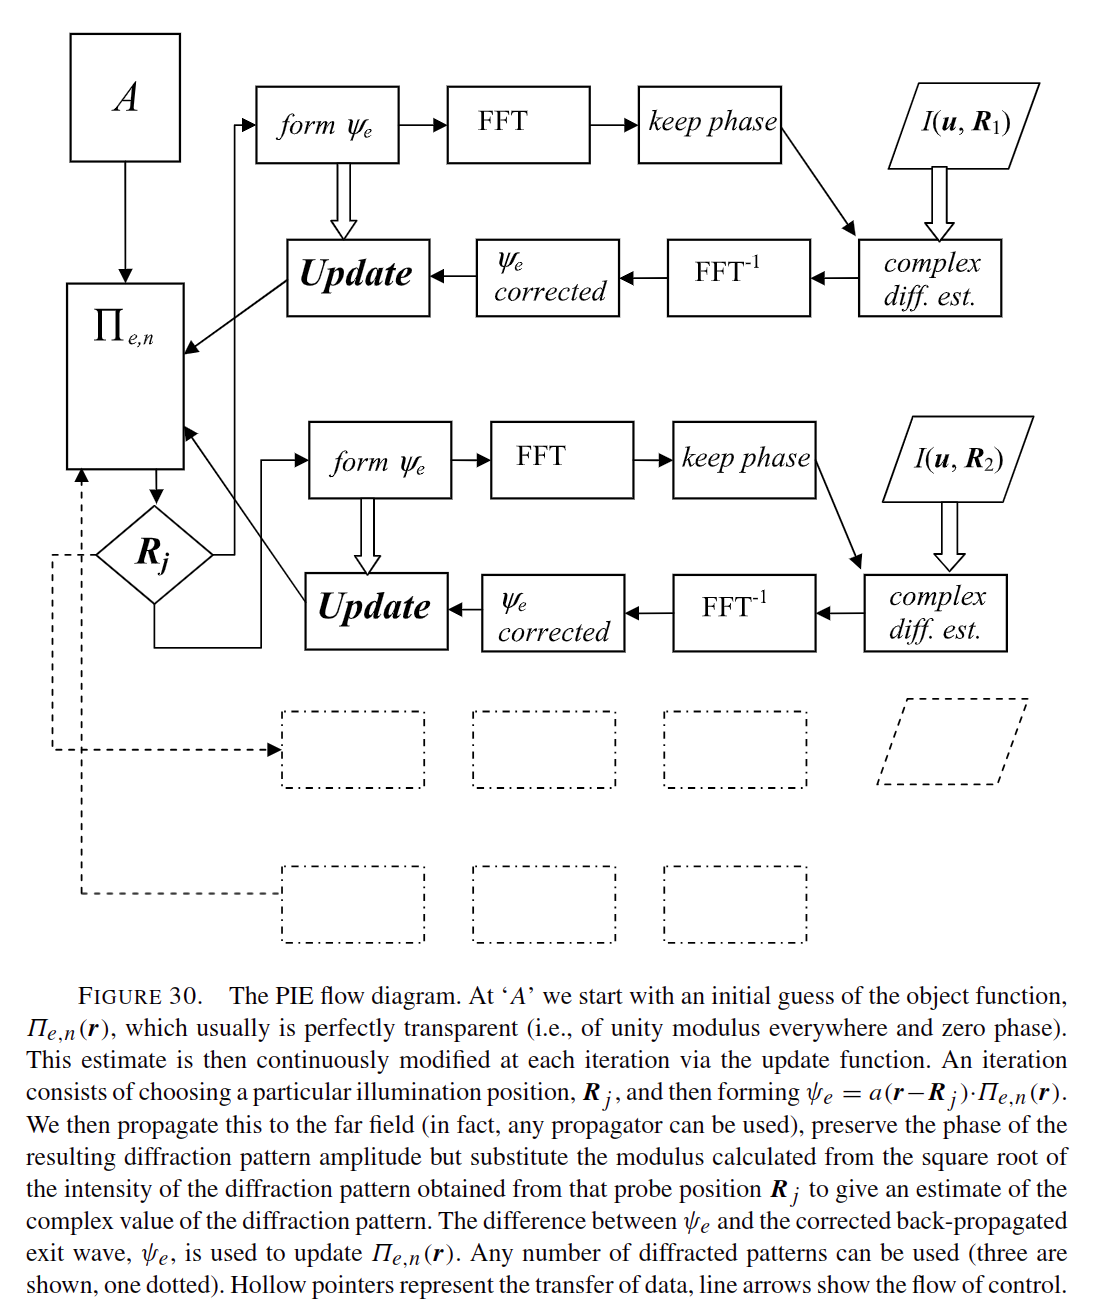
\includegraphics[width=\textwidth]{figures/PIE_diagram.png}

\section{\cite{Rodenburg2004-oi} \citenum{Rodenburg2004-oi}}

Here, Rodenburg uses a different nomenclature, namely
\begin{equation}
    \psi(\bm{r},\bm{R})=O(\bm{r})P(\bm{r}-\bm{R}),
\end{equation}
and notes that it doesn't matter whether the object function $O(\bm{r})$ or illumination function $P(\bm{r})$ is moved, as long as the shift occurs relative to one another with distance $\bm{R}$. If the shape of $P(\bm{r})$ is not accurately known, the phase-retrieval algorithm will still work, though with a less accurate end result. Therefore, it might be advised to measure the incident probe in the object plane.

In this paper, the update function itself as well as its parameters $\alpha$ and $\beta$ are explained. The update function is crucial to the success of the algorithm, since it makes the effective deconvolution that occurs possible.


\section{\cite{Maiden2009-pn} \citenum{Maiden2009-pn}}

Iterative phase-retrieval is one method of recovering a complex-valued reconstruction of a sample from measurement of its diffraction pattern. This is achieved by \textit{a priori} knowledge of system contraints, e.\,g. nonnegativity, realness, atomicity and the requirement that the reconstructed image is zero valued outside of a finite region.

For good results with PIE, an overlap of $60-70\%$ is required. In this paper, an extended PIE (``ePIE") algorithm is introduced. Now, both $O_0(\bm{r})$ and $P_0(\bm{r})$ are guessed and updated in a analogous fashion (see PIE). The updating process continues for $J$ diffraction patterns until a single ePIE iteration has been completed. 

The scanning grid was generated using randomized grid distances, since periodic grids can lead to a periodic pattern appearing in the reconstruction. The initial probe function $P_0(\bm{r}$ was guessed as a circular support function. This probe estimate was not updated until the first iteration had been completed (in comparison to 20 iterations in pPIE). It was shown that ePIE converges very fast and is resilient to Poisson noise and (somewhat) inaccurate guesses of $P_0(\bm{r})$.

An experimentally estimable definition of the normalised error is introduced given by
\begin{equation}
    E_\Psi =\frac{\sum_{j}^{} \sum_{\bm{u}}^{} |\sqrt{I_j(\bm{u})}-|\Psi_j(\bm{u})||^2}
    {\sum_{j}^{} \sum_{\bm{u}}^{} I_j(\bm{u})}.
\end{equation}
End results were even improved by some kind of error reduction algorithm involving projections between the two contraint sets without any relaxation or reflection of the projections.





\section{\cite{Popoff2009-xs} \citenum{Popoff2009-xs}}
The authors introduce  a  method  to  experimentally  measure  the  monochromatic  transmission  matrix (TM)  of  a  complex medium in optics.
The mesoscopic TM of an optical system for a given wavelength is defined as the matrix $K$ of the complex coefficients $k_{mn}$ connecting the optical field (in amplitude and phase) in the $m^{th}$ output free mode to the one in the $n^{th}$ input free mode. Therefore, the projection $E_m^{out}$ of the outgoing optical field on the $m^{th}$ free mode is given by
\begin{equation}
    E_m^{out}=\sum_n k_{mn} E_n^{in},
\end{equation}
where $E_n^{in}$ is the complex amplitude of the optical field in the $n^{th}$ incoming free mode.

The studied sample is a \SI{80+-20}{\micro m} thick deposit of ZnO.

After measuring the TM, the authors were able to utilize the conjugate transpose $K^\dagger$ to optain a localized (focused) target output vector $E^{target}$ using
\begin{equation}
    E^{in}=K^\dagger E^{target}.
\end{equation}
The experimental result of this \textit{monochromatic phase conjugation focusing} is shown here:

\noindent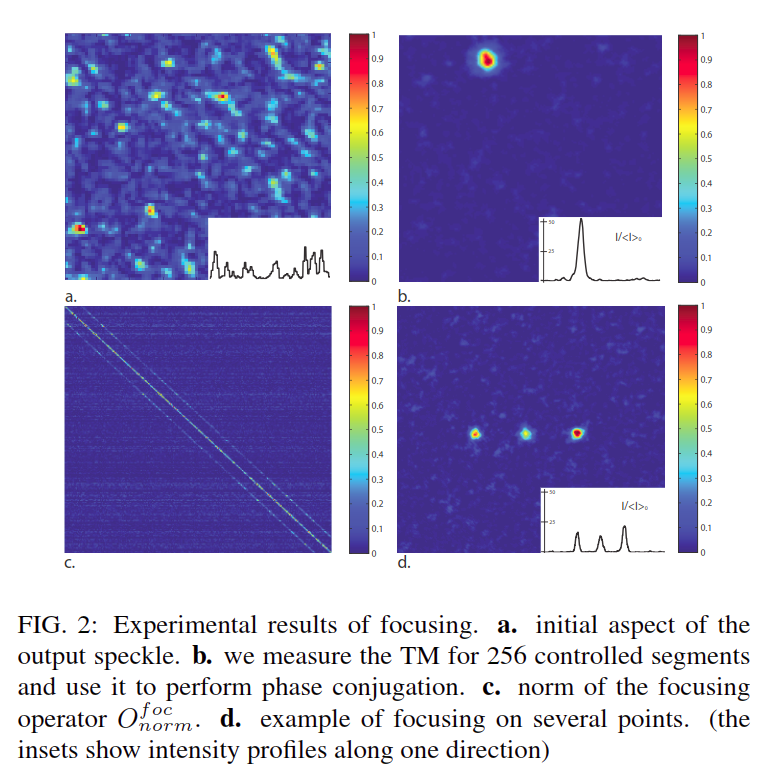
\includegraphics[width=0.9\textwidth]{figures/TM_conjugate.png}

\section{\cite{Pai_Bosch_Mosk_2018} \citenum{Pai_Bosch_Mosk_2018}}

They use a slightly different nomenclature
\begin{equation}
    E^{out}=T E^{in},
\end{equation}
with transmission matrix $T$. Its elements are measured in a spatioal basis set by scanning the incident beam and recording the corresponding transmitted fields. The open closed transmission channels of the medium can then be found by \textit{singular value decomposition}  of the transmission matrix. 

A hexagonal spiral laser scan is used to optain the ($M \times N$) TM, which results in faster scanning speed and less noise (the alternative is using a SLM). The number $N$ translates to the number of laser spots scanned on the incident sample surface (roughly of the size of an Airy disk) and $M$ is the number of camera pixels used for detection.

Since the incident spots are spatially independend, the TM can be constructed column-wise by a step-by-step approach:
\\

\noindent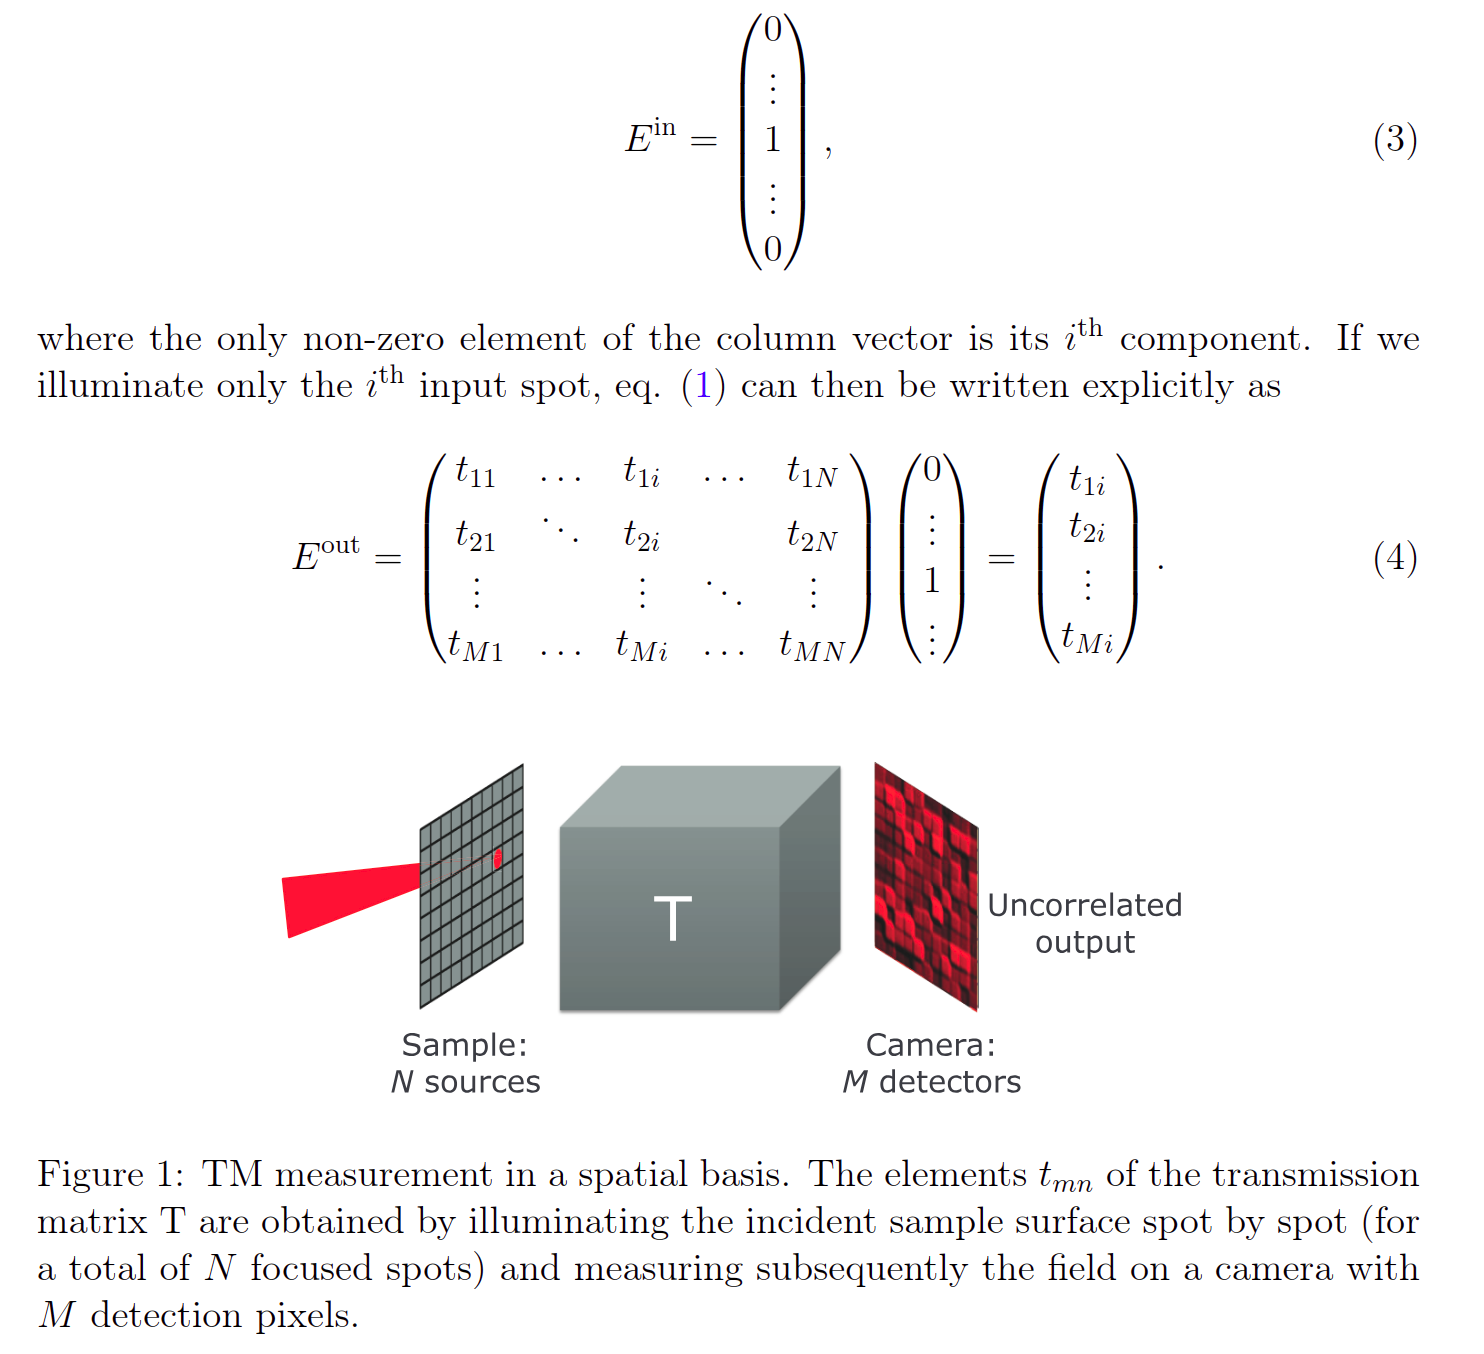
\includegraphics[width=\textwidth]{figures/TM_measurement.png}

The measurement apparatus is shown and explained in Figure 2.

\noindent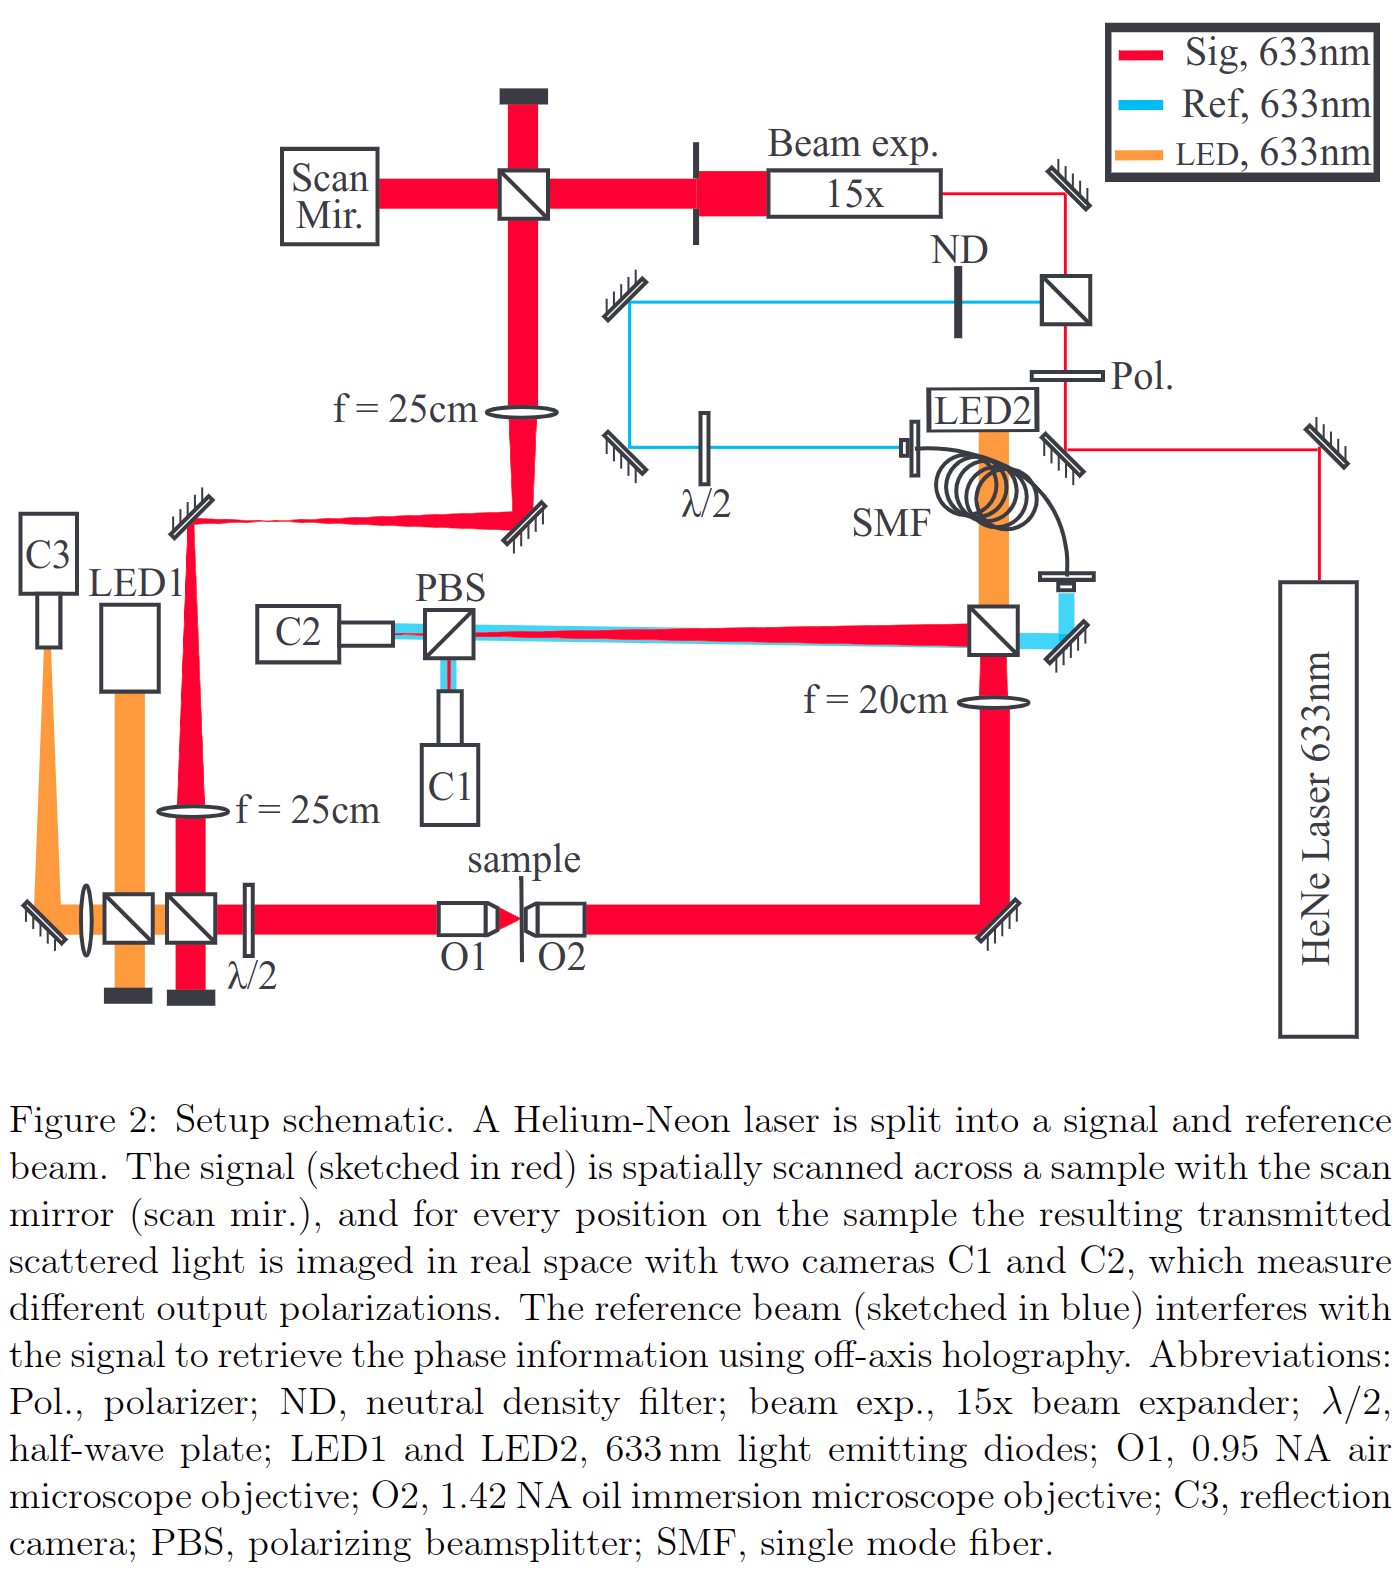
\includegraphics[width=0.9\textwidth]{figures/TM_setup.png}

The scattered light field is detected using off-axis holography. The sample is separately illuminated by horizontally ($H$) and vertically ($V$) polarized light, which provides a full picture of the TM in the form
\begin{equation}
    T=
    \left[ {\begin{array}{cc}
   T_{HH} & T_{HV} \\
   T_{VH} & T_{VV} \\
  \end{array} } \right].
\end{equation}



\section{\cite{Maiden2010-un} \citenum{Maiden2010-un}}

The authors use a entirely lensless setup and record the diffraction patterns in the Fresnel region (at \SI{19}{mm} distance to the sample) to improve convergence and solve image ambiguities. To mitigate the problem of a very bright central spot by undiffracted components a diffuser is used.
The overlap is about \SI{70}{\percent} with random offsets to avoid ambiguities.


\section{\cite{Huang2014-yo} \citenum{Huang2014-yo}}
Using a Fermat spiral drastically improves SNR of both amplitude and phase retrieval (experimentally between 80 and 150 \%). This may be explained by low symmetrie (which is ideal for ptychography) and a high uniformity of the overlaps.

The scanning pattern determines the real-space sampling conditions: the overlap ratio and the overlap uniformness. It was shown that regular periodicity in a mesh scan will cause periodic artifacts in the reconstructed images (``raster grid pathology"). \textit{Concentric patterns} break the translational symmetry, but can not compete with Fermat spirals in terms of uniform overlaps.



\section{\cite{Bouchet2017-hk} \citenum{Bouchet2017-hk}}

Chapter 6 discusses the fundamental limit on the precision of position and lifetime in STORM/PALM measurements.
The lower bound of the estimations is assessed by calculating the \textit{Cramér-Roa lower bound} on the variance of position and decay rate estimators. 

In statistics, an \textbf{estimator} is a rule for calculating an estimate of a given quantity based on observed data: thus the rule (the estimator), the quantity of interest (the estimand) and its result (the estimate) are distinguished. Suppose there is a fixed parameter $\theta$  that needs to be estimated. Then an estimator is a function that maps the sample space to a set of sample estimates. An estimator of $\theta$  is usually denoted by the symbol $\hat{\theta}$.
The \textbf{variance} of $\hat{\theta}$ is simply the expected value of the squared sampling deviations; that is, $\mathrm{var}(\hat{\theta}) =\mathrm{E} [(\hat{\theta}-\mathrm{E} [\hat{\theta}])^{2}]$. It is used to indicate how far, on average, the collection of estimates are from the expected value of the estimates.
The \textbf{bias} of $\hat{\theta}$ is defined as $B(\hat{\theta })=\mathrm{E}(\hat{\theta})-\theta$. It is the distance between the average of the collection of estimates, and the single parameter being estimated. 


\section{\cite{Maiden2013-zp} \citenum{Maiden2013-zp}}

Since ptychography is able to reconstruct the object and probe functions without any \textit{a priori} knowledge about them, using a diffuser yields two distinct advantages:

\begin{enumerate}
    \item The usually high-intensity zero-order component of the illumination (unscattered light) is attenuated, leaving us with a lower dynamic range (which is easier to handle).
    \item Enhancing the phase diversity of the probe was shown to improve the quality of the reconstructed image.
\end{enumerate}

\section{\cite{Maiden2011-up} \citenum{Maiden2011-up}}

Exploiting the information redundancy (due to overlap) in ptychography, the authors achieve superresolution of a factor 3 (in comparison to the aperture of the recording device).
Two lenses have been used in the experimental setup.


One of three core principle is a 4x extrapolation of the computated diffraction pattern in comparison to the extend of the recorded part.
The new superresolution reconstruction process (SR-PIE) is based on ePIE, but extrapolates the recorded diffraction images beyond the aperture of the detector.

\section{\cite{Vellekoop2007-ke} \citenum{Vellekoop2007-ke}}

We determine the optimal phase for a
single segment at a time by cycling its phase from 0 to 2$\pi$. For each segment we store the phase at which the target intensity is the highest. At that point the contribution of the segment is in phase with the al- ready present diffuse background. After the measure- ments have been performed for all segments, the phase of the segments is set to their stored values. Now the contributions from all segments interfere constructively and the target intensity is at the glo- bal maximum.

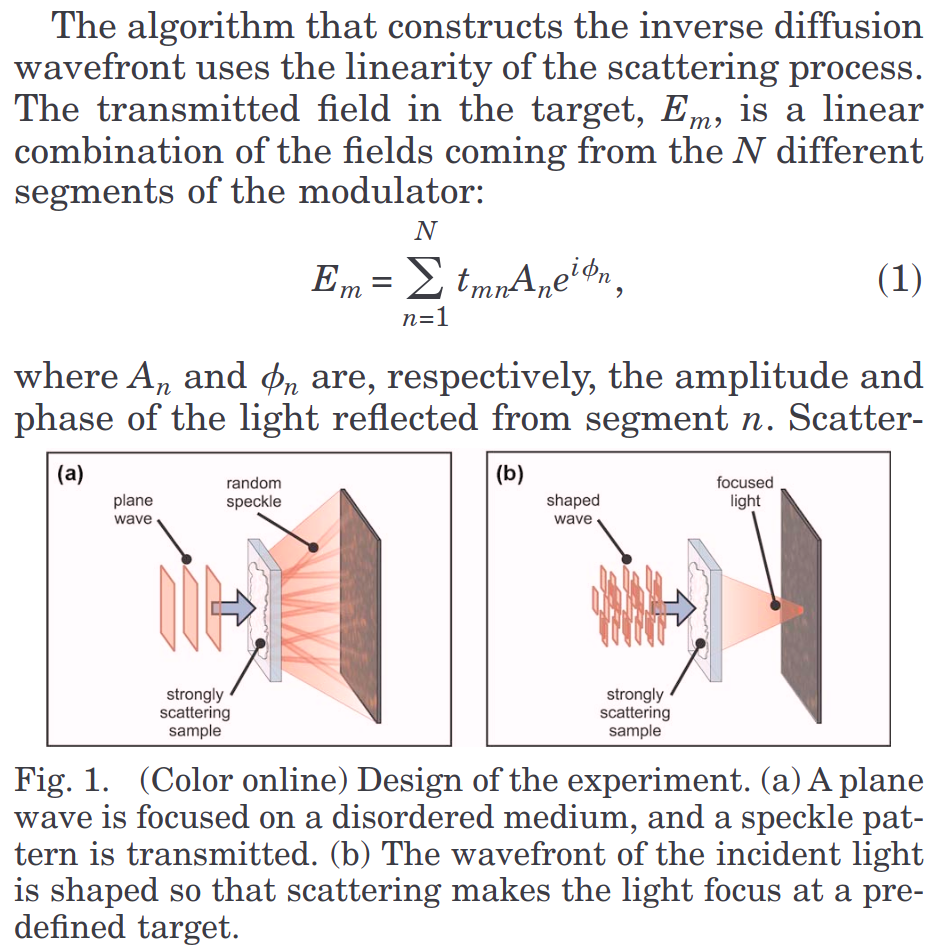
\includegraphics[width=.8\textwidth]{figures/FL.png}


\section{\cite{Anand2010-ji} \citenum{Anand2010-ji}}
This is the first paper for our weekly journal club.
The authors describe a method of recording speckle patterns in a 3D volume and iteratively reconstructing a complex-valued object (solving the phase problem). An object is illuminated with plane waves and behind the object lies a random amplitude mask to generate higher spatial frequencies which was beneficial for the reconstruction algorithm.

\section{\cite{Eglese1990-dv} \citenum{Eglese1990-dv}}
Stimulated Annealing (SA) is a optimization algorithm derived from the physical analogy of the annealing of solids. For example, one would heat a solid into a liquid to remove former defects in a crystal structure (global minimum of possible energy states). Then, by cooling the liquid slowly in the vicinity of its freezing point, the liquid that is comprised of randomly ordered atoms has enough time to crystellize evenly and without defects. If it is cooled down to quickly, stochastical local defects (local minima) will appear.

In comparison to simple descent algorithms, SA is robust to high incidences of local minima (at least when they are no very deep) and comprises a useful tool to find global minima in difficult optimization problem while being easily implemented. The algorithm works as follows:

\begin{itemize}
    \item Select initial state $i \in S$ (solution space).
    \item Select initial temperature $T>0$
    \item Set temperature counter $t = 0$
    \item Outer loop over cooling schedule $T = T(t)$
    \item Inner loop: generate state $j$, a neighbour of $i$
    \item Calculate $\delta = f(j) - F(i)$
    \item if $\delta < 0$ then $i = j$
    \item elseif random(0, 1) < exp($-\delta/T$) then $i = j$
    \item iterate over neighbors and temperatures, until T = 0.
\end{itemize}

Important for an efficient asymptotic convergence to the global minimum is the choice for the cooling schedule as well as the neighbourhood structure. 
It has been shown that SA always converges successfully for infinitely slow cooling schedules.


\section{\cite{Maiden2017-iz} \citenum{Maiden2017-iz}}

The paper gives a good overview of ptychography in the year 2017. Particularly interesting is the literature on correcting positioning errors, e.g. with \textbf{simulated annealing} \cite{Maiden2012-bj}. Then, this paper revisits the (original) PIE family of algorithms and shows how to improve robustness and convergence rate by adding two modifications. In ePIE, an improvement in acquiring a non-trivial (diversivied) probe function arises. Furthermore, the authors borrow the idea of \textbf{momentum from the machine learning community}. For simulated data, a 20-fold improvement in convergence over ePIE has been demonstrated.

\subsection{Overview of Operation}
For every single iteration of ePIE, the authors shuffled the order in which the diffraction patterns are analyzed. A distinction of the pixel pitch in the object and probe estimates ,$\Delta_\mathrm{r}$, is made for the method used for propagation.
For far-field propagation using the Fourier transform,

\begin{equation}
    \Delta_\mathrm{r} = \Big(\frac{\lambda z}{M\Delta_{c}}, \frac{\lambda z}{N\Delta_{c}}\Big),
\end{equation}
and in the near-field using the angular spectrum,
\begin{equation}
    \Delta_\mathrm{r} = (\delta_\mathrm{c}, \delta_\mathrm{c}).
\end{equation}

The original choice for the \textbf{ePIE object update function} is insightfully explained on page 738.

\subsection{mPIE}

mPIE stands for \textbf{momentum PIE} and is an extension of regularized PIE (rPIE) which incorporated regularization to the update function to account for bright and dim areas of the object. It was shown that among the family of PIE algorithms (PIE, ePIE, rPIE, mPIE) performed best in terms of convergence speed, robustness and reconstruction error. However, mPIE suffers from the addition of more hyperparameters. A table with (empirically established) recommended parameters is provided (Table 3). In Figure 3, the idea of \textbf{ptychographical momentum} is sketched.

\begin{center}
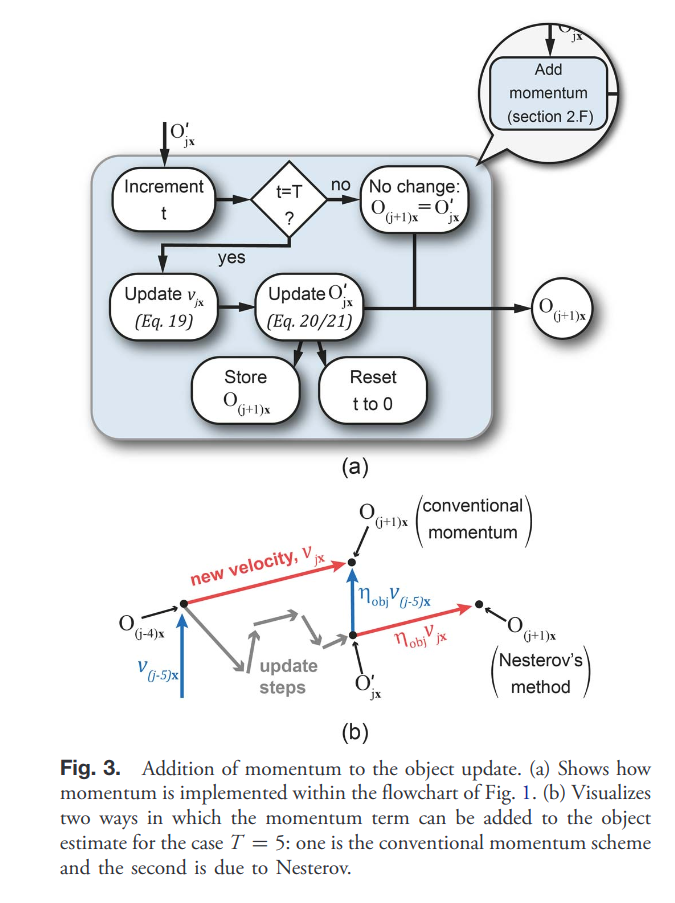
\includegraphics[width=0.8\textwidth]{figures/mPIE_momentum.png}
\end{center}

\section{\cite{Loetgering_undated-wt} \citenum{Loetgering_undated-wt}}

Theoretically, ptychographic coherent diffraction imaging allow an infinite field of view (FOV) in scanned specimen. Since the FOV is practically limited by computer memory, the authors introduced a compression algorithm for diffraction data denoted by $I \in R^{M\times N}$, where $M$ is the number of detector pixels and $N$ is the number of scan positions.
The compression is then achieved by aproximating the diffraction data by a rankK truncated singular value decomposition (SVD):
\begin{equation}
    I \approx USV',
\end{equation}

where $U \in R^{M \times K}$, $S \in R^{K \times K}$ and $V \in R^{N \times K}$ (the apostrophe denotes the conjugate transpose). The compression rate is then given as $K/ N$. The results after 1000 iterations of ePIE are shown in Figure 2.

\begin{center}
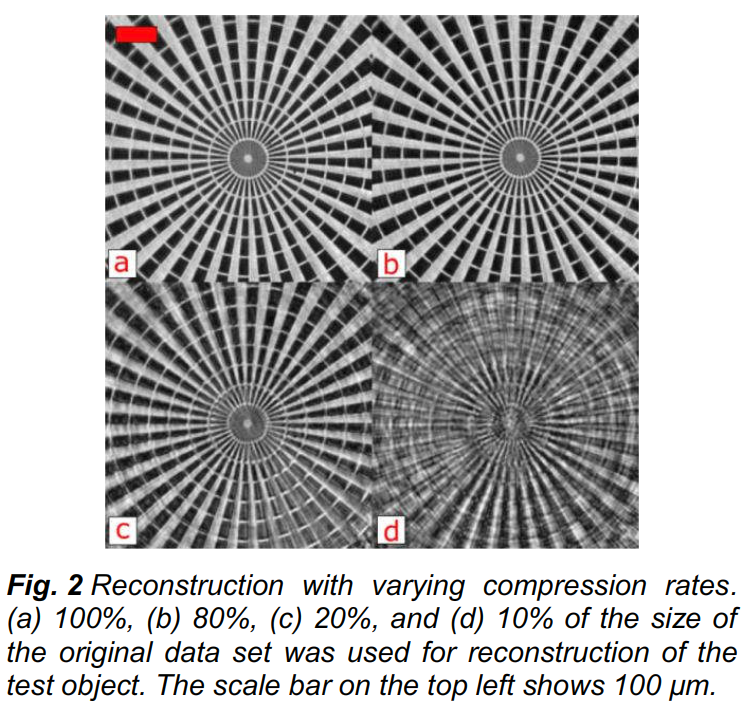
\includegraphics[width=0.65\textwidth]{figures/compression_ePIE.png}
\end{center}

Furthermore, instead of averaging multiple exposures to increase the SNA of the diffraction patterns, the authors describe a method of stitching them together to achieve a dynamical range of 20 bit.

\section{\cite{Loetgering2017-re} \citenum{Loetgering2017-re}}

This is a more comprehensive work based on the previous paper by Lars Lötgering \citenum{Loetgering_undated-wt}. In chapter 2.5, an \textbf{assessment for the resolution in ptychography} is established using the area under curve of a Fourier ring correlation.

\newcite{Parrent1966-au}
 
The basic entity in the theory of partial coherence is the mutual coherence function $\Gamma_{12}(\tau)$:

\begin{equation}
      \Gamma_{12}(\tau) = (x_1, x_2, \tau) = \langle V(x_1,t) V^*(x_2, t+\tau)\rangle.
\end{equation}

Here, $x$ denotes the position vector and the sharp brackets indicate a long time average. The complex degree of coherence is here defined as the normalized coherence function. The tratment of problems involving partially coherent light involves the solution of two wave equations with $\Gamma_{12}(\tau)$.

If the path distances $c\cdot \tau$ are suitably small, we can rewrite the mutual coherence function as the \textbf{mutual intensity function}
\begin{equation}
    \Gamma(x_1,x_2) = \Gamma_{12} = \Gamma(x_1,x_2,0)
\end{equation}
which reduces the wave equations to two Helmholtz equations
\begin{equation}
    \nabla_s \Gamma_{12}+k^2\Gamma_{12} = 0 \,\,\,\, (s = 1,2).
\end{equation}

Now, two principal theorems emerge:

\begin{enumerate}
    \item A field is coherent if and only if the mutual intensity function describing it can be factored in the form
    \begin{equation}
        \Gamma_{12} = U(x_1)U^*(x_2)
    \end{equation}
    where 
    \begin{equation}
        \nabla_s U(x_1)+k^2U(x_1) = 0.
    \end{equation}
    \item An incoherenct field cannot exist in free space; however, an incoherent source consistent with this result may be defined.    
\end{enumerate}

\newcite{Thibault2013-kg}

The authors present that the problem of partially coherent illumination (either caused by the source or other decoherent systems like vibrating or mixed samples) in ptychography can be overcome by the assumption of wide-sense stationary statistics that can be described by low-rank density matrices. As a results, it is possible to reconstruct modes in the illumination or, shown in simulations, quantum system states in an Ising model.


\newcite{Guizar-Sicairos2012-rq}
The spacial-frequency spectrum is important for the quality of ptychographical reconstructions.


\newcite{MacKay2004-to}
\subsection{Chapter V: Neural Networks}


\newcite{Kamilov2015-lp}
\subsection*{Reading goal}
Demetri Psalti's and Ulugbek Kamilov's paper describe a similar approach to my current reseach question. This makes it detremental to understand their work and probably cite them in the future.
\subsection*{Content}
The authors demonstrate a neural-network-based algorithm for solving the phase retrieval problem in tomography. Off-axis holography under 80 illumination angles is applied. The object is separated in 420 slices which are represented as forward beam propagation layers in a neural network. The error between the predicted hologram and its measurement is then used in conjunction with a conventional backpropagation technique to optimize for the object (in a basis of pixels).
The only sparsity constraint seems to be that the index perturbation is real and positive (no further prior knowledge due to the pixel basis). The results are compared to conventional tomography techniques that fail mainly due to their dependence on the Born approximation (single scattering). The learning-based method converges to the same results no matter how the object was initialized (constant or with three different conventional tomography results).

\newcite{Goldsborough2016-fz}
\subsection*{Reading Goal}
Get a better technical understanding of the toolkit TensoFlow, the computational paradigms behind tensors, the logic of stateful dataflow graphs etc.\\
Along the way, I want to look for new ideas regarding our PtychoKeras project.
\subsection*{Content}
ML algorithms is TensorFlow are represented as computational graphs (or dataflow graphs). They are comprised of \textit{nodes} (describing operations) and \textit{edges} (representing data that flows between these operations).
``Any operation must be backed by an associated implementation which is referred to as the operation's \textit{kernel}''.
The edges that represent data flowing are referred to as \textit{tensors}. Tensors themselves do not store values in memory.\\
In graph computing, \textit{Common Subgraph Elimination} is employed to accelerate operations that would be executed multiple times (by truncating redundancies in the graph). The ability of defining while-loops is discussed briefly in a paragraph about \textit{Control Flow}.


\newcite{Waller2015-ec}
\subsection*{Reading Goal}
Get an overview of comparable work to my PhD project.

\subsection*{Content}
This article is a review of \cite{Kamilov2015-lp} which is described earlier. Furthermore, the future and problem of provability in computational imaging (based on ANNs) are discussed.

\printbibliography
\end{document}
